%!TEX root = ../../soulexchange.tex

\begin{post}
	\postdata{A fortnight}{2011}{9}{13}{1}{48}{46}
	\begin{content}
Splendid! Two awesome weeks that felt like at least a month. Last week the classes have (finally) started. In the first half of the semester I am taking 4 classes — two "real" (Growth Strategy and Valuation of IT Media Business) and two "exchange" (Korean for Foreigners I and Korean Business and Culture). This should keep me relatively busy, but still leave some time for fun and traveling and other things exchange students usually do. The class schedule here is quite interesting. Classes are only 80 minutes long, and there are usually two each weak (Mon+Wed or Tue+Thu). Out of class work seems to be less extensive than in Delft so in general the workload might be lower. However, it has still been only a week, so I don't want to make premature conclusions.

I have to say that I am more than happy with my choice of subjects. I picked the courses so they would support my current direction, because I did not want to spend this semester doing meaningless courses just to bring some ECTS home.

%[caption id="attachment_39" align="aligncenter" width="500" caption="Tha hikin&#039; gang"]<a style="text-decoration:underline;font-family:'Helvetica Neue', Helvetica, Arial, sans-serif;" href="http://soulexchange.files.wordpress.com/2011/09/p1000274.jpg"><img class="size-large wp-image-39" style="background-image:initial;background-attachment:initial;background-color:#eeeeee;margin-top:.4em;border-color:initial;border-style:initial;" title="Tha gang" src="http://soulexchange.files.wordpress.com/2011/09/p1000274.jpg?w=300" alt="" width="500" height="333" /></a>[/caption]
%\begin{figure}
%\centering
%\setlength{\fboxsep}{0pt}
%\setlength{\fboxrule}{0.5pt}
%\fbox{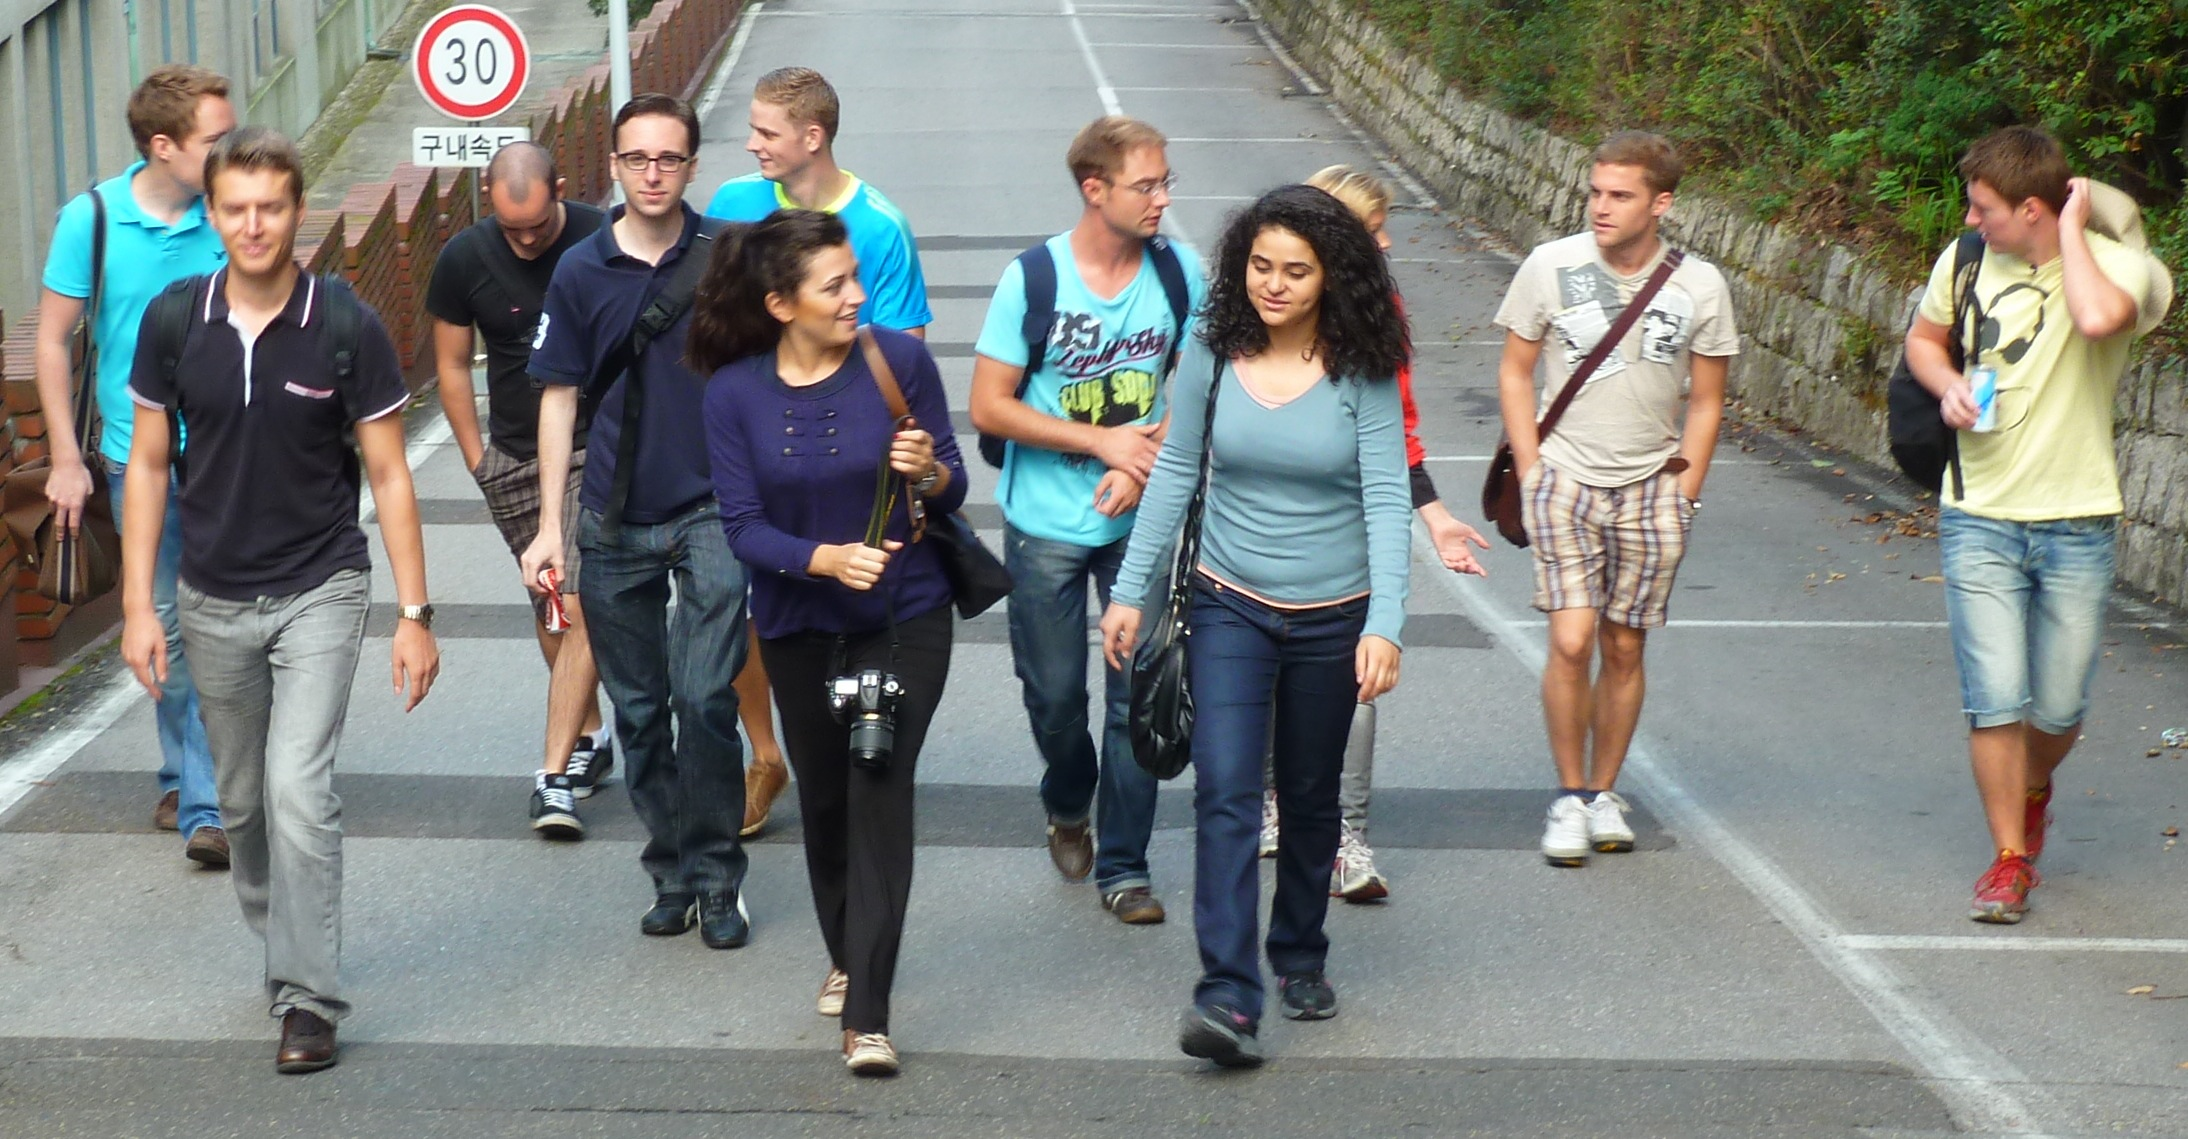
\includegraphics[width=0.4\textwidth]{photos/09/13/p1000274.jpg}}
%%\vspace{-25pt}
%%\caption{Tha hikin' gang}
%\label{default}
%\end{figure}

\begin{wrapfigure}{r}{0.41\textwidth}
\centering\vspace{-12pt}
\fbox{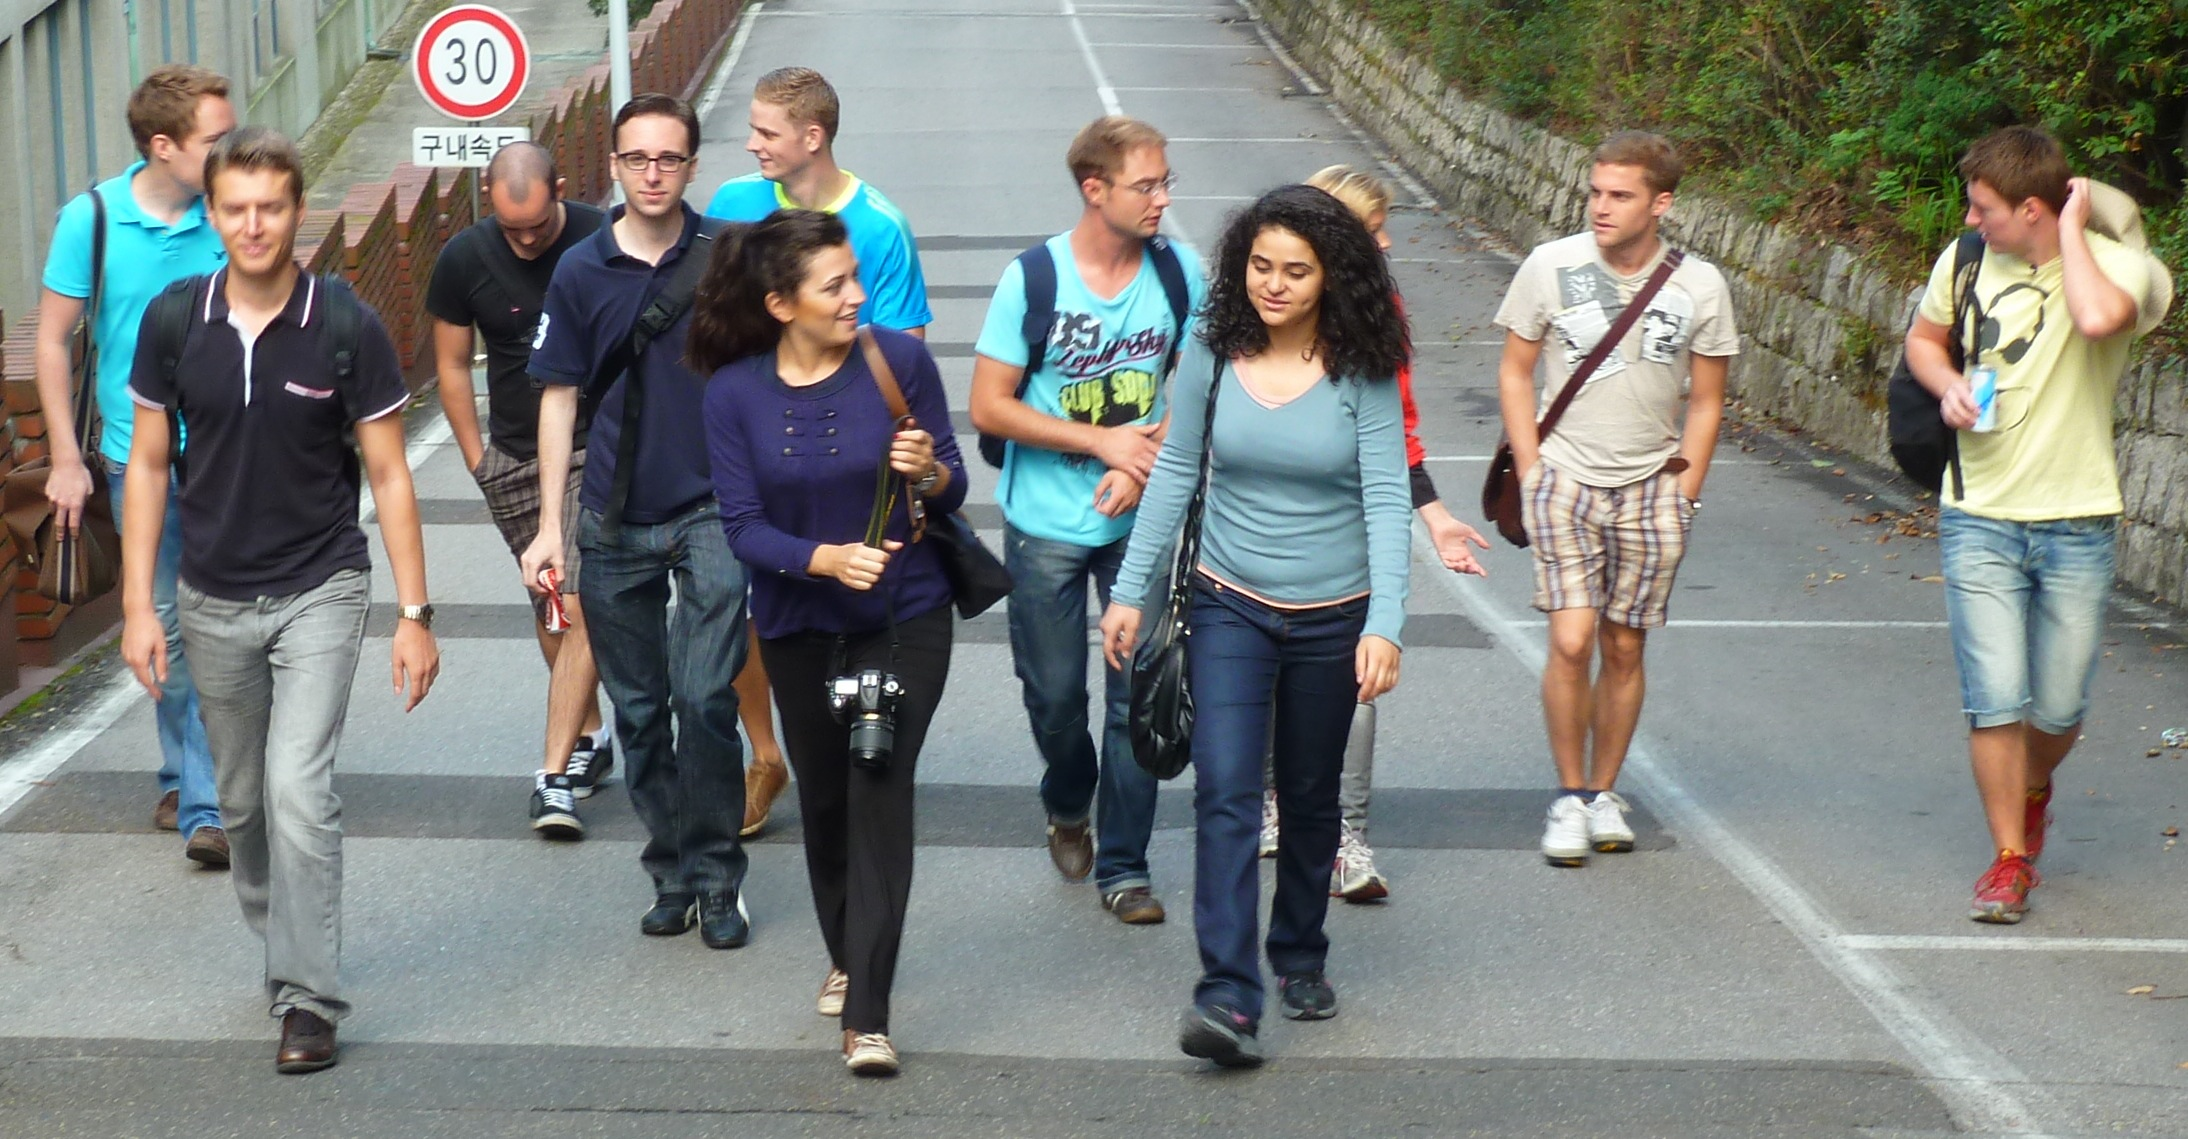
\includegraphics[width=0.4\textwidth]{photos/09/13/p1000274.jpg}}
\vspace{-8pt}
\caption*{Tha hikin' gang}
\vspace{-25pt}
\end{wrapfigure}Enough of school, though. As announced earlier, on Saturday we went to the Bukhansan National Park for some hiking. Well, Korean hiking is certainly different from the European. It all started with about 300m of altitude of stairs. Yes, steep stairs like in a mall. On the left from the stairs there was a wall, on the right there was a fence and a military area with forbidden access. Fun fun fun. Unfortunately, thanks to all the smog, the view on Seoul was not very god either, so we just had to keep climbing up.

%\begin{wrapfigure}{R}{0.25\textwidth}
%%\centering
%\vspace{-26pt}
%\setlength{\fboxsep}{0pt}
%\setlength{\fboxrule}{0.5pt}
%\fbox{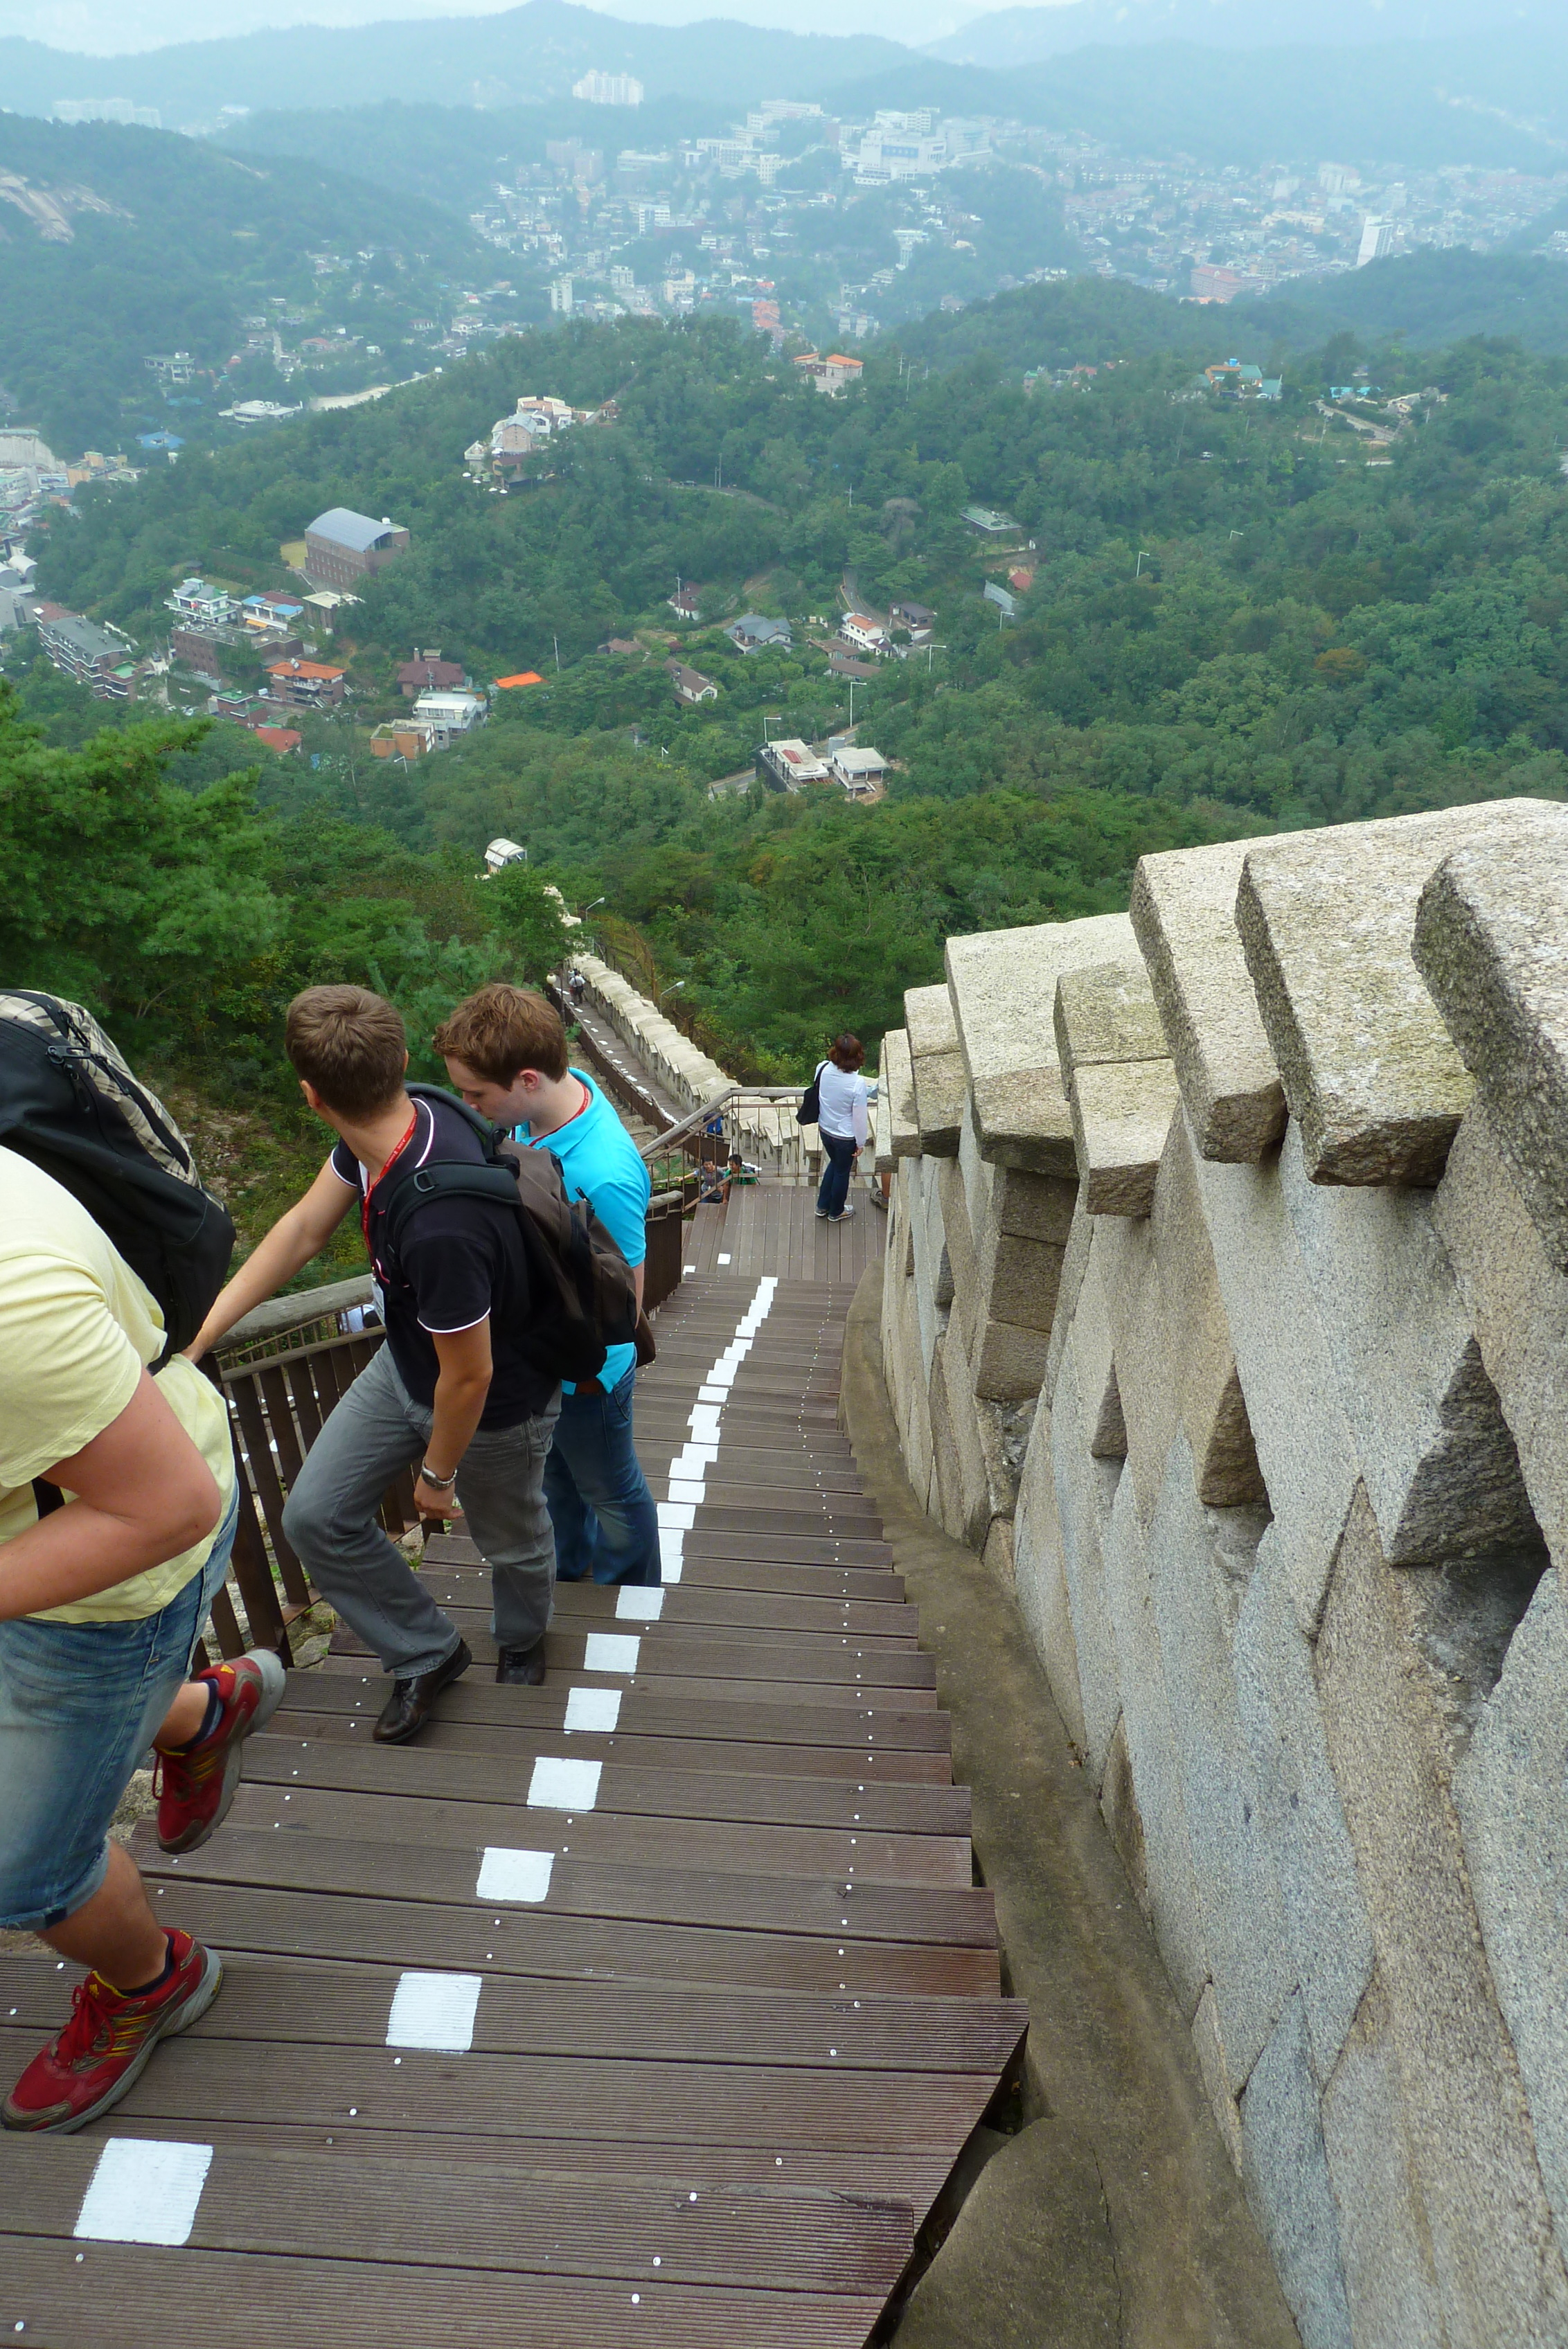
\includegraphics[width=0.25\textwidth]{photos/09/13/p1000296.jpg}}
%\vspace{-25pt}
%%\caption{Tha hikin' gang}
%\label{default}
%\end{wrapfigure}

%[caption id="attachment_42" align="aligncenter" width="333" caption="Stairway To Heaven"]<a href="http://soulexchange.files.wordpress.com/2011/09/p1000296.jpg"><img class="size-medium wp-image-42" title="Stairway To Heaven" src="http://soulexchange.files.wordpress.com/2011/09/p1000296.jpg?w=200" alt="" width="333" height="500" /></a>[/caption]

Funny thing about this national park is that since it is close to some military facility, every visitor has to fill out a entry form and gets a badge. In the form there is a list of rules such as "Photographs can be takes only at designated spots" and "No alcoholic beverages can be consumed inside the park" etc. Sounds like a exciting trip, right. Well, so we kept climbing until we got to the top. There was a small plain with a lot of Koreans, that were having lunch, and few security guards that were taking care that no one is breaking the aforementioned rules.

%<p style="text-align:center;"><a href="http://soulexchange.files.wordpress.com/2011/09/p1000286.jpg"><img class="aligncenter size-medium wp-image-40" title="Badge" src="http://soulexchange.files.wordpress.com/2011/09/p1000286.jpg?w=300" alt="" width="500" height="333" /></a></p>

The rest of the trip fortunately went better. Even though the whole was basically between the fence and the wall, the nature around was more interesting and once we even reached some kind of a pine groove that allowed us to walk next to the stairs like real hikers. Yeah!

\begin{figure}[h]
\centering
\subfigure[The badge]{
\raggedleft
\fbox{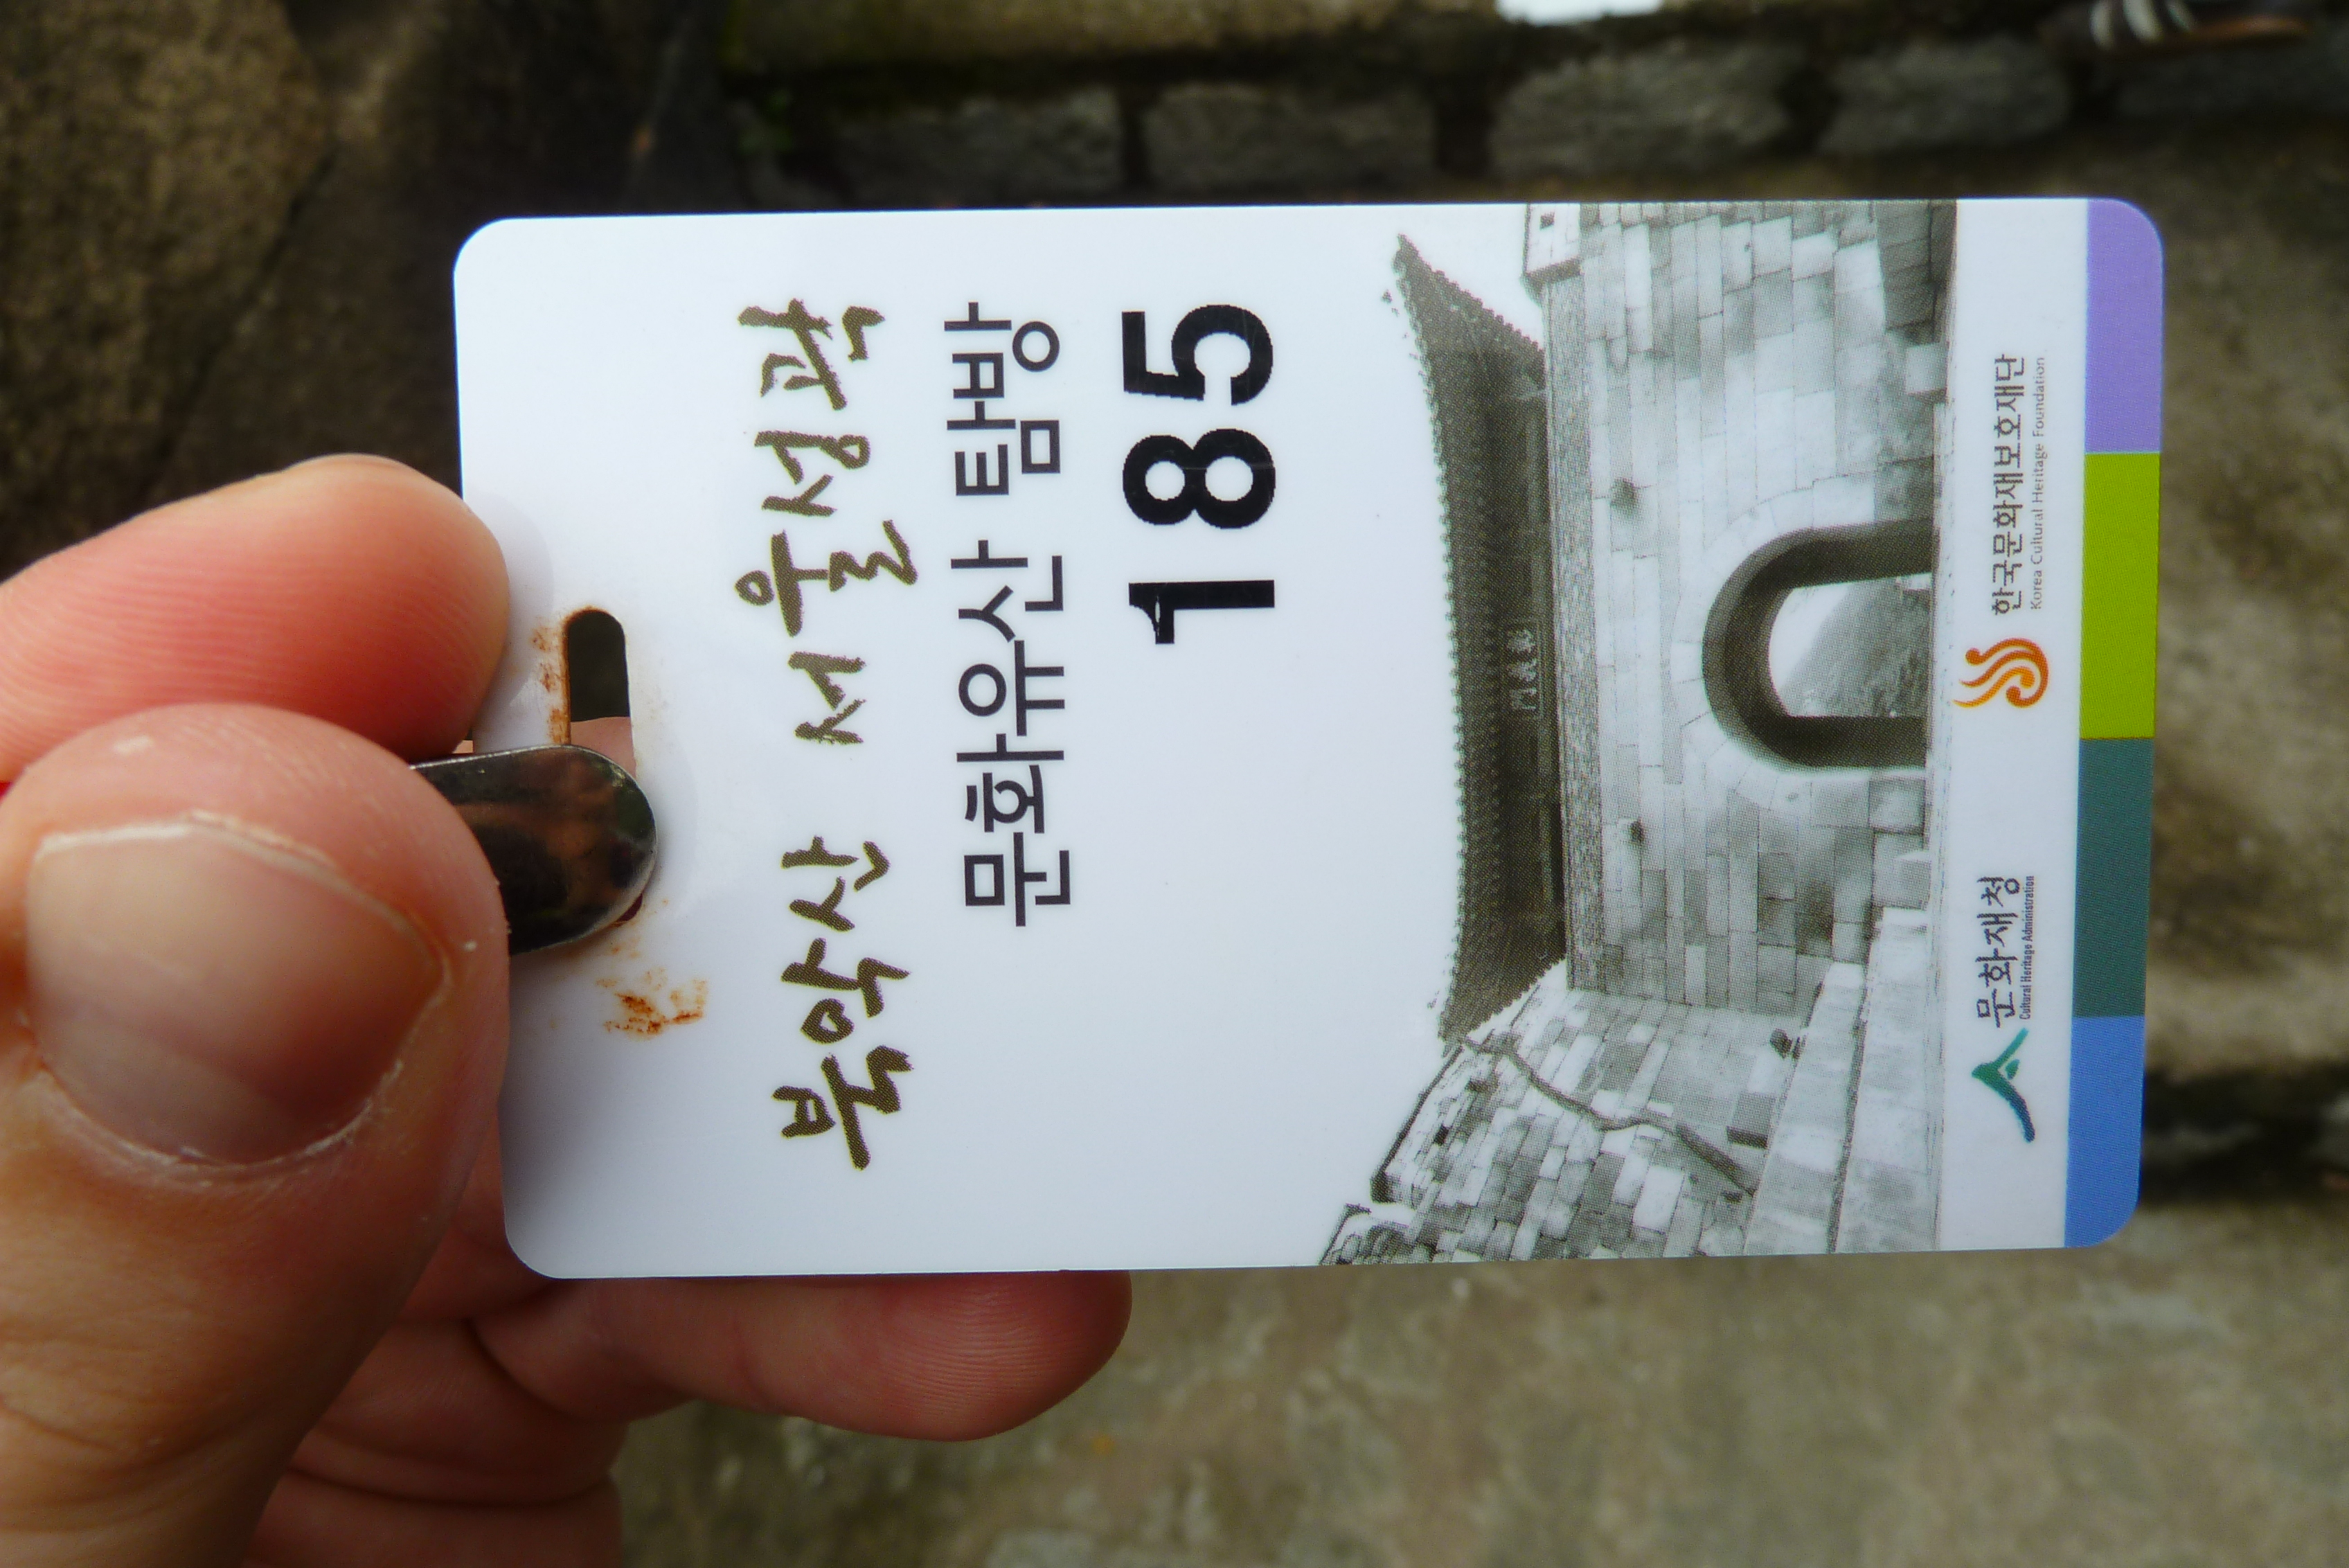
\includegraphics[width=0.42\textwidth]{photos/09/13/p1000286.jpg}}
}
\subfigure[Lunching on the top]{
\raggedright
\fbox{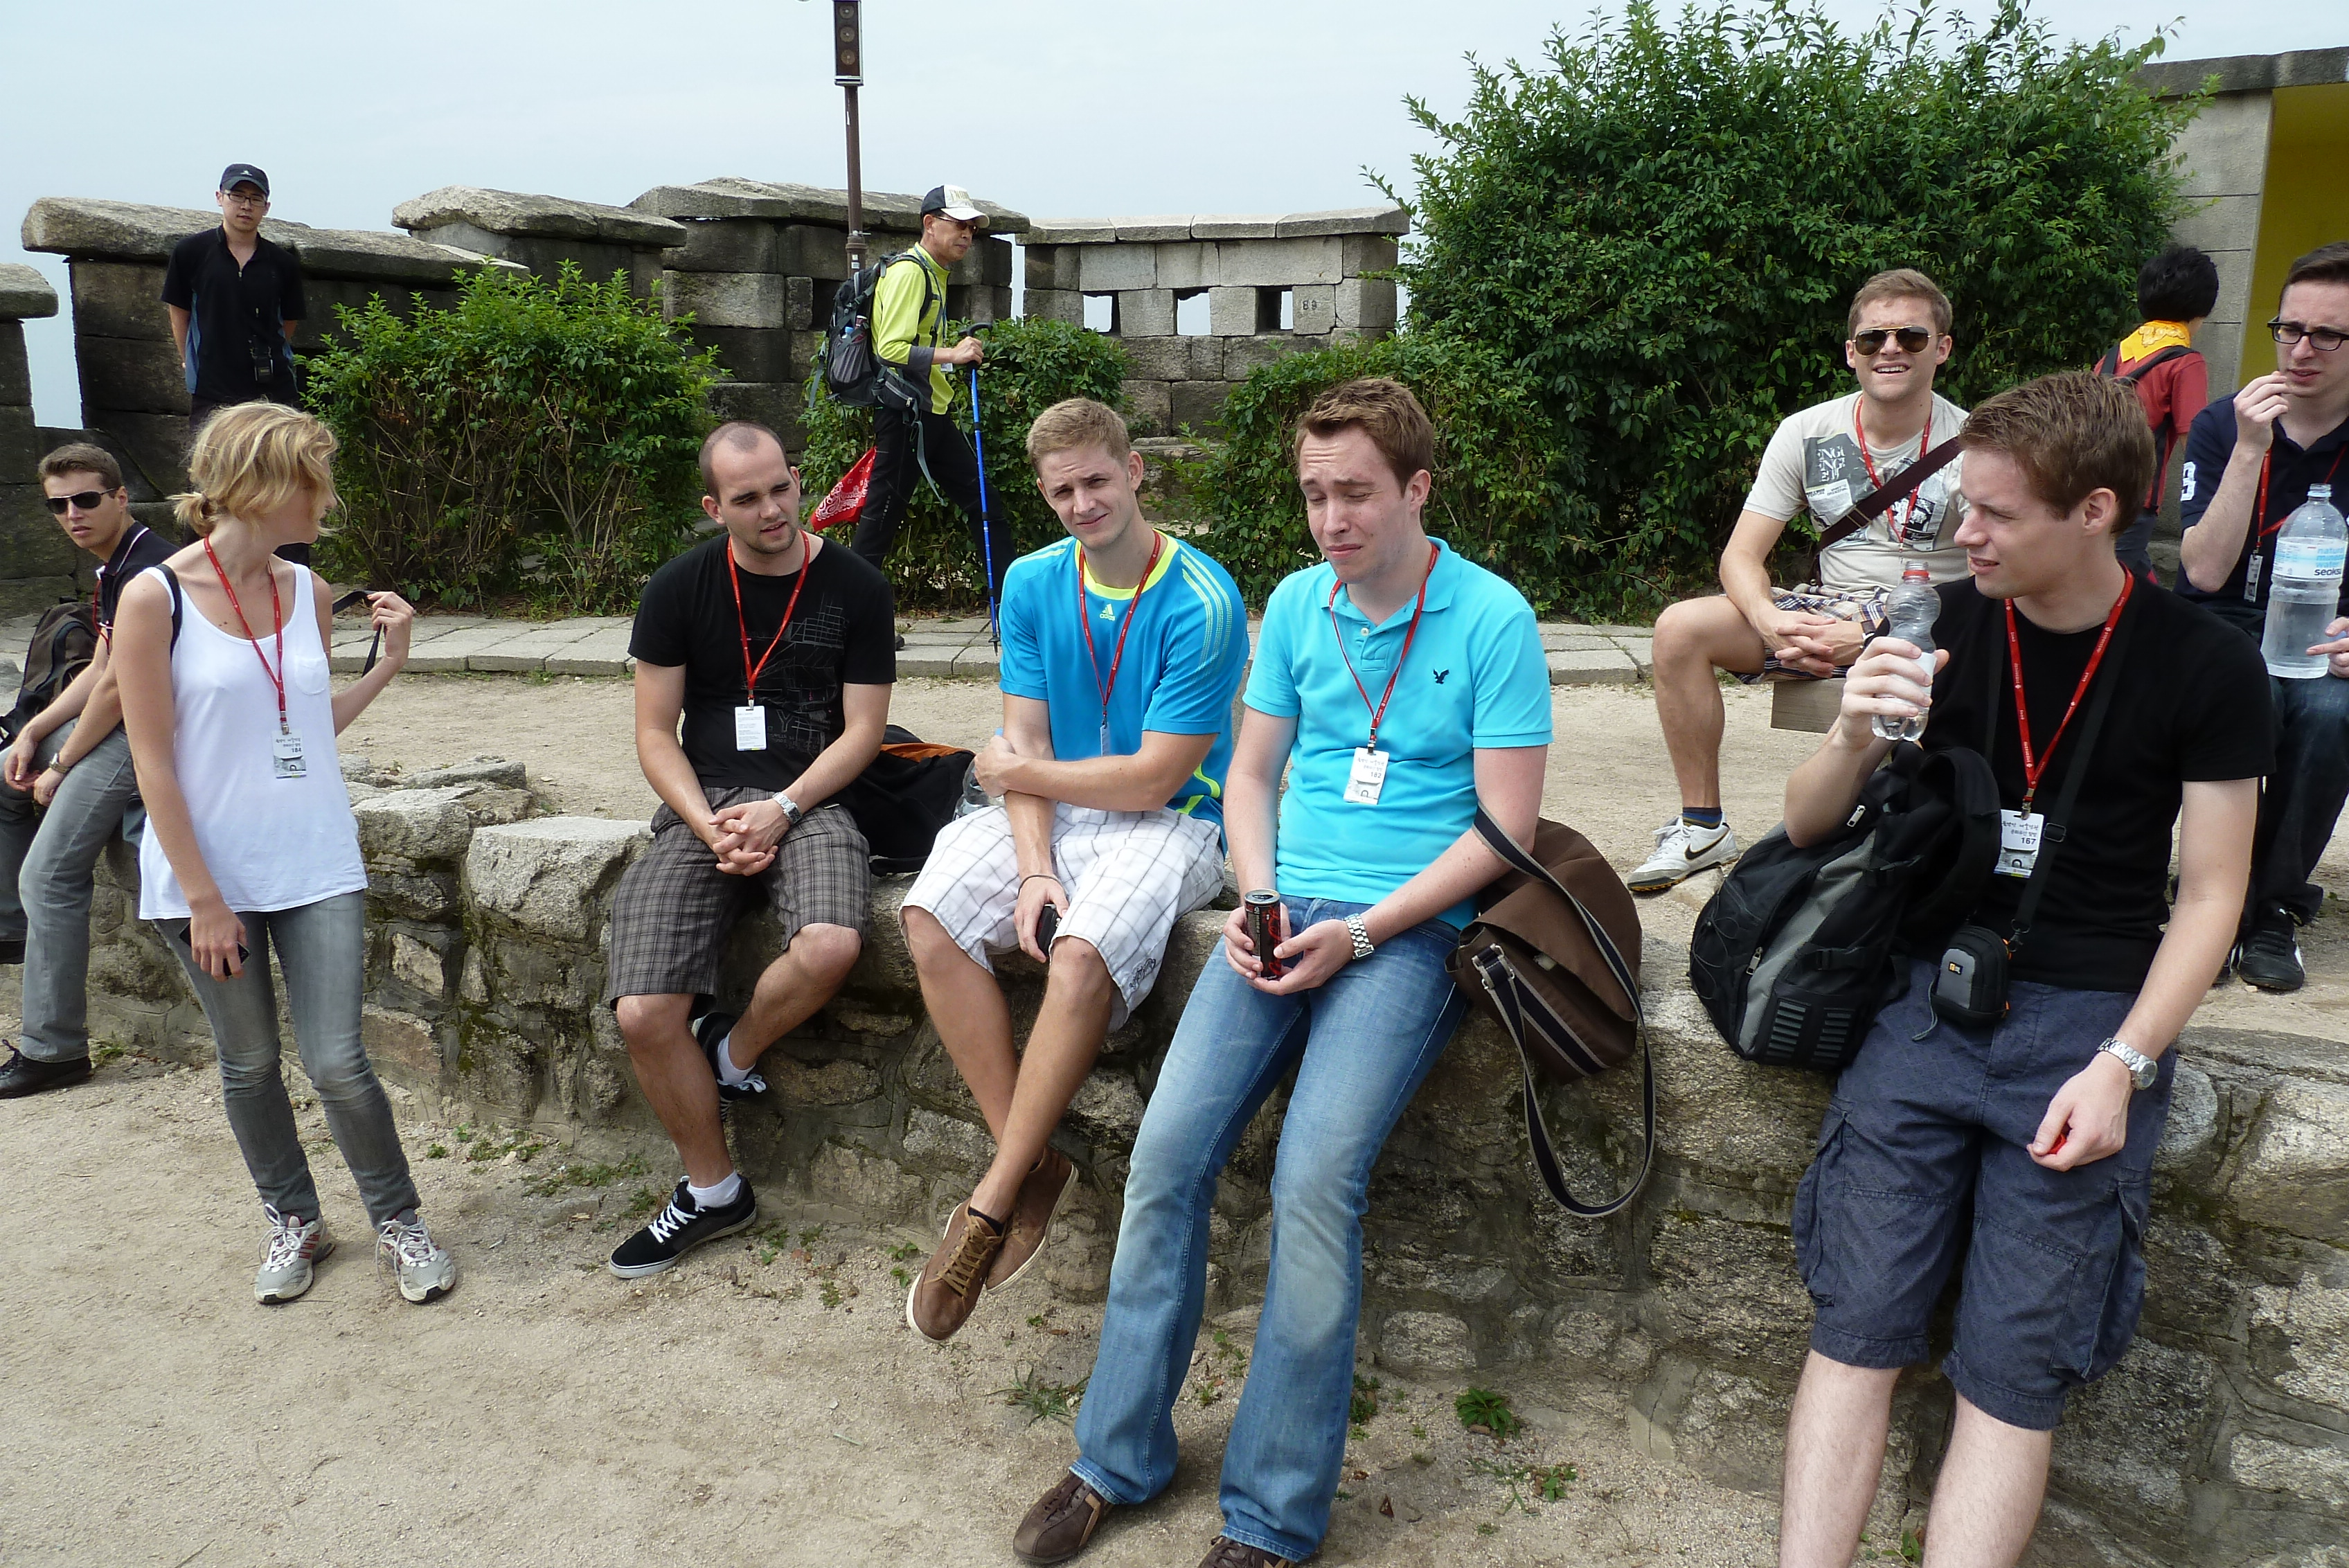
\includegraphics[width=0.42\textwidth]{photos/09/13/p1000314.jpg}}
}
\end{figure}

%[caption id="attachment_43" align="aligncenter" width="5000" caption="Lunching at the top"]<a href="http://soulexchange.files.wordpress.com/2011/09/p1000314.jpg"><img class="size-medium wp-image-43 " title="Lunching at the top" src="http://soulexchange.files.wordpress.com/2011/09/p1000314.jpg?w=300" alt="" width="5000" height="333" /></a>[/caption]

\begin{wrapfigure}{l}{0.41\textwidth}
\centering\fbox{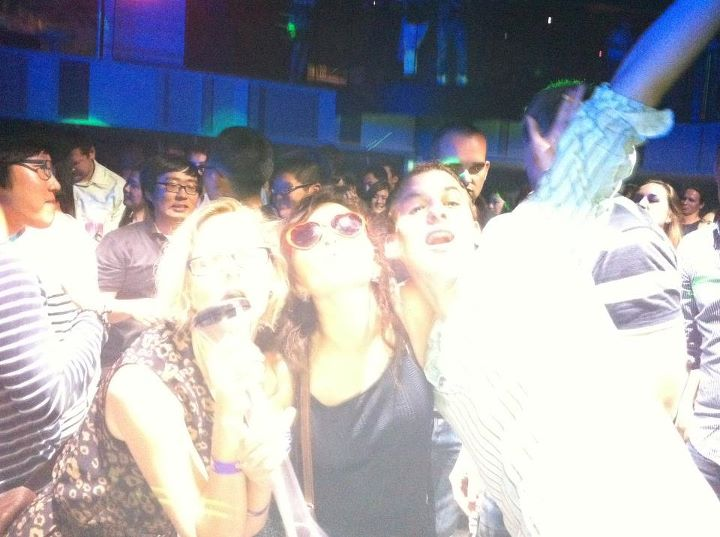
\includegraphics[width=0.4\textwidth]{photos/09/13/club.jpg}}
\vspace{-6pt}
\caption{Keep dancing till the world ends...}
\vspace{-12pt}
\end{wrapfigure}In the evening we were planning to go clubbing to Gangnam's Club Eden. Eden is supposed to be the biggest/most famous/bestest club in Seoul / Korea / Asia / World / Universe, so we wanted to experience it as well. Our plan did not quite work out, because we ended up in Itaewon in Club Volume, where we did not have to pay the cover to get in. Well, the party was nice, even though I liked the Cocoon Club a little more. From unknown reasons I prefer mostly Korean clubs, because otherwise I feel like in some European city. Since Itaewon is quite and international part of Seoul, the club was full of intl's, including a Dutch girl from R'dam, who's parents were living in Prague. After coming home at 7am we had a quick breakfast with Rik and Lauriane at the roof of our dorms and then off to bed for 9 hours of well deserved sleep. It's quite funny that I basically went to bed in European time, since 7am here is 12pm in Europe.

\end{content}
\end{post}
